\begin{exercise}
Υπολογίστε στο επίπεδο τον μετασχηματισμό στροφής γωνία $\theta = \cfrac{\pi}{3}$ γύρω από το σημείο $P = (4,1)$

Στην συνέχεια, γράψτε ένα script σε \texttt{Julia} όπου θα υπολογίζει τον παραπάνω πίνακα μετασχηματισμού μέσω πολλαπλασιασμών των βασικών μετασχηματισμών και εφαρμόστε τον, στο παρακάτω σχήμα  σχεδιάζοντας στο ίδιο γράφημα και το αρχικό και το μετασχηματισμένο.

\begin{figure}[hbt]
  \begin{center}
	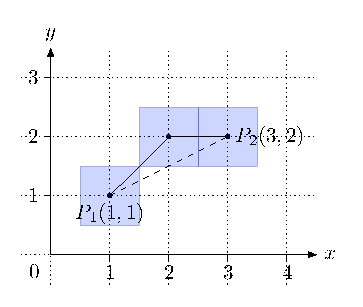
\includegraphics[scale=1]{Chapter1/Exercises/ex17/graph1.pdf}
  \end{center}
%  \caption{Παράσταση ζητούμενων ευθυγ\textcolor{red}{what}ράμμων τμημάτων}
\end{figure}

\end{exercise}


%\begin{solution}
%
%΄Εστω ότι έχει φωτισθεί το $pixel$ $(x_{i}, y_{i})$. Επειδή βρισκόμαστε στην περιοχή 1 το επόμενο προς φωτισμό $pixel$ θα είναι το $(x_{i-1}, y_{i+1})$ ή το $(x_{i-1}, y_{i})$ .
%
%\begin{figure}[hbt]
%  \begin{center}
%	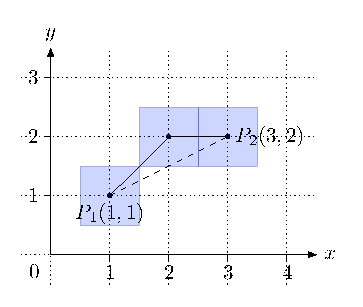
\includegraphics[scale=0.7]{Chapter1/Exercises/ex17/graph1.pdf}
%  \end{center}
%%  \caption{Παράσταση ζητούμενων ευθυγ\textcolor{red}{what}ράμμων τμημάτων}
%\end{figure}
%
%
%\begin{align*}
%    \begin{tikzpicture}[x=1cm, y=1cm]
%    \draw[step=3cm, line width=0.5mm, gray!10!gray] (0,0) grid (\width,\hauteur); 
%      \node[anchor=north] at (1.5,0) {\Large $x_{i-1}$};
%      \node at (1.5,4.5) {\Huge $C$};
%      \node at (1.5,1.5) {\Huge $B$};
%      \node at (4.5,4.5) {\Huge $D$};
%      \node[anchor=east] at (0,3) {\huge $M$};
%      \node[anchor=east] at (0,1.5) {\Large $y_{i}$};
%      \node[anchor=east] at (0,4.5) {\Large $y_{i+1}$};
%      \node[anchor=north] at (4.5,0) {\Large $ x_{i}$};
%      \draw [pattern={Lines[angle=45,distance=4pt,]},pattern color=orange]  (4.5,1.5) circle [radius=1.5];
%      \draw (4.8,0) arc [x radius=4.8, y radius=4.2, start angle=0, end angle=90];
%      \draw (4.8,0) arc [x radius=4.8, y radius=2.7, start angle=0, end angle=90];
%      \foreach \x in {1.5,4.5} {
%            \node [fill= gray, fill opacity=0.1, draw=none, thick, minimum size=3cm] at (\x,4.5);
%            \node [fill= gray, fill opacity=0.1, draw=none, thick, minimum size=3cm] at (\x,1.5);
%            }
%      \draw [decorate,
%            decoration = {brace,mirror}] (0.1,3.02) --  (0.1,4.18)
%            node[pos=0.5,right=2pt,black]{$e_i$};      
%    \end{tikzpicture}
%\end{align*}
%\begin{gather*}
%    f_{mid2,i+1} = b^2 (x_{i}-1-1)^2 + a^2 (y_{i+1}+\frac{1}{2})^2 -a^2 b^2 = 
%    \\ = \underbrace{b^2 (x_{i}-1)^2 + a^2 (y_{i}+\frac{1}{2})^2 -a^2 b^2}_\text{$f_{mid2,i}$} -a^2 (y_{i}+\frac{1}{2})^2 -2b^2 x_{i-1} + b^2 + a^2 y^2_{i+1} + a^2 y_{i+1} + \frac{a^2}{4} = 
%    \\ = f_{mid2,i} - a^2 (y_{i}+\frac{1}{2})^2 -2b^2 (x_{i}-1) + b^2 + a^2 y^2_{i+1} + a^2 y_{i+1} + \frac{a^2}{4}= 
%    \\ = f_{mid2,i} - a^2 y^2_{i} - a^2 y_{i} - \frac{a^2}{4} -2b^2 (x_{i}-1) + b^2 + a^2 y^2_{i+1} + a^2 y_{i+1} + \frac{a^2}{4} = 
%    \\ = f_{mid2,i} + a^2 (y^2_{i+1} - y^2_{i}) + a^2 (y_{i+1} - y_{i}) -2b^2 (x_{i}-1) + b^2.
%\end{gather*}
%\begin{center}
%    \begin{tabular}{ |c|c| } 
%        \hline
%        $f_{mid2,i}<0$ &$ f_{mid2,i} -2b^2 (x_{i}-1) + b^2 + 2a^2 y_{i+1}$\\
%        \hline
%        $f_{mid2,i} \geq 0$ &$ f_{mid2,i} -2b^2 (x_{i}-1) + b^2 $\\
%        \hline  
%    \end{tabular}
%\end{center}
%Άρα έχουμε ότι ο αναδρομικός τύπος του $f_{mid2,i}$ είναι:
%\begin{gather*}
%   f_{mid2,i+1} = f_{mid2,i} + a^2 (y^2_{i+1} - y^2_{i}) + a^2 (y_{i+1} - y_{i}) -2b^2 (x_{i}-1) + b^2.
%\end{gather*}
%\end{solution}